% CVPR 2027 submission draft -- gated recursive self-improvement for VLA policies (preregistered study)
\documentclass[10pt,twocolumn,letterpaper]{article}

\usepackage[review]{cvpr}      % REVIEW version (line numbers, anonymous). Final: \usepackage{cvpr}
%% This file contains a number of tweaks that are typically applied to the main document.
%% They are not enabled by default, but can be enabled by uncommenting the relevant lines.


%%
%% Official support for 2-column teaser figure
%%
\usepackage{cuted} %< for strip environment

%%
%% For auto-referencing of figures (see fig/teaser.tex and \label{} therein) 
%%
\usepackage{currfile} %< for \currfilebase macro

%%
%% caption and (global) spacing overrides
%%
\usepackage{caption} %< for "\captionof" commands (teaser)
% \setlength{\abovecaptionskip}{.5em} % space above caption
% \setlength{\belowcaptionskip}{1em} % space below caption

%%
%% Inline annotations; for predefined colors, refer to "dvipsnames" in the xcolor package:
%% https://tinyurl.com/overleaf-colors
%%
\newcommand{\red}[1]{{\color{red}#1}}
\newcommand{\todo}[1]{{\color{red}#1}}
\newcommand{\TODO}[1]{\textbf{\color{red}[TODO: #1]}}
%%
%% Disable for camera ready / submission by uncommenting these lines:
%%
% \renewcommand{\TODO}[1]{}
% \renewcommand{\todo}[1]{#1}

%%
%% Work harder in optimizing text layout. Typically shrinks text by 1/6 of page, enable
%% it at the very end of the writing process, when you are just above the page limit.
%%
% \usepackage{microtype}

%%
%% Fine-tune paragraph spacing.
%%
% \renewcommand{\paragraph}[1]{\vspace{.5em}\noindent\textbf{#1.}}

%%
%% Globally adjusts space between figure and caption.
%%
% \setlength{\abovecaptionskip}{.5em}

%%
%% Allows "the use of \paper to refer to the project name"
%% with automatic management of space at the end of the word.
%%
% \usepackage{xspace}
% \newcommand{\paper}{ProjectName\xspace}

%%
%% Commonly used math definitions.
%%
% \DeclareMathOperator*{\argmin}{arg\,min}
% \DeclareMathOperator*{\argmax}{arg\,max}

%%
%% Tighten underline.
%%
% \usepackage{soul}
% \setuldepth{foobar}

%%
%% Reconfigure paragraph (tweaks spacing)
%%

\usepackage{booktabs}
\usepackage{enumitem}
\usepackage{algorithm}
\usepackage{algorithmic}
\usepackage{amsmath,amssymb}
\usepackage{graphicx}
\graphicspath{{fig/}{./}}
\definecolor{cvprblue}{rgb}{0.21,0.49,0.74}
\usepackage[pagebackref,breaklinks,colorlinks,allcolors=cvprblue]{hyperref}
\usepackage[capitalize,nameinlink]{cleveref}

\def\confName{CVPR}
\def\confYear{2027}

\title{Letting a Robot Train Itself: What Helps, What Doesn't, and What Only Looks Like It Helps}

\author{Anonymous CVPR submission\\
Paper ID \cvprPaperID}

\begin{document}
\maketitle
\begin{figure}[t]
  \centering
  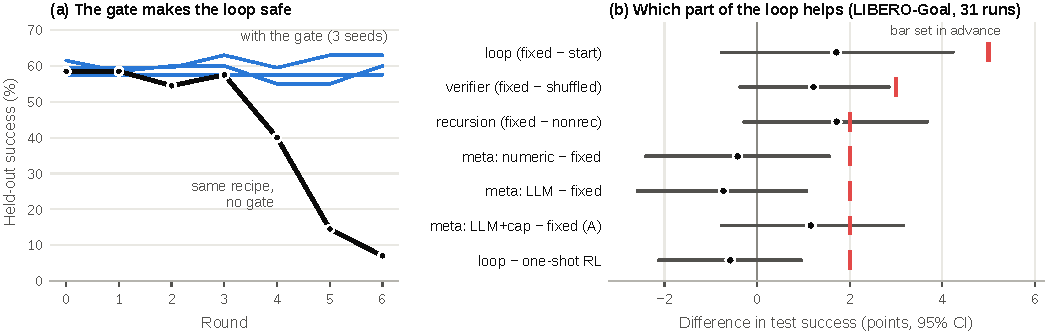
\includegraphics[width=\linewidth]{fig_teaser}
  \caption{\textbf{A robot policy that trains on its own attempts.} (a) One practice placement of a LIBERO-Spatial task and two attempts by the initial OpenVLA-OFT policy, shown as its camera saw them. The simulator's success check labels each attempt, and the loop trains on such labelled attempts. (b) LIBERO-Goal, behaviour cloning on the policy's own samples. When every new version is accepted, success on the round's 200 held-out placements falls from 58.5\% to 7\% within six rounds. When a version is kept only if it does not regress on fresh paired placements, the same recipe stays at its starting level.}
  \label{fig:teaser}
\end{figure}
\begin{abstract}
Recursive self-improvement (RSI) promises a policy that practises on tasks it writes for itself, keeps only what an external verifier confirms, and revises its own training procedure. We ask whether this promise holds for vision-language-action (VLA) policies, and whether any gain is due to the recursive and meta-level parts of the loop rather than to plain reinforcement learning. We build a framework in which every ingredient is a switch: a verifier gate that accepts or rejects each new version on fresh held-out placements, recursion (practice generated by the latest policy or frozen at the initial one), a verifier (real or permuted success labels), a meta level (none, numeric search, or an LLM that diagnoses round records and edits the training procedure inside a declared space), and a compute-matched one-shot RL baseline. All claims were preregistered with sealed official tests, public amendments, and replicate-averaged reads. On LIBERO-Goal with OpenVLA-OFT (31 runs, four seeds, two GPU platforms) the gated loop never degrades a policy and gains $+1$ to $+2$ points; recursion contributes $+1.7$ points (95\% CI $[-0.3, +3.7]$) and the verifier $+1.2$ $[-0.4, +2.9]$, but neither reaches its preregistered bar, and no meta-level variant beats a fixed, hand-tuned procedure (all within $\pm 1.2$ points; the same null on a second, separately registered study). We show why: the object-level loop reaches the same plateau under every procedure in the space, so there is nothing for a meta level to fix, even though the LLM's diagnoses are correct. The meta level only becomes distinguishable from RL when the starting procedure fails; a preregistered self-repair study (sealed, to be read on 2026-11-08) tests exactly that. In a second domain (code world models, four LLMs), the same loop gives verified-feedback gains of $+2.6$ to $+7$ points and recursion is significant at eight rounds ($+2.8$ $[+1.2, +4.5]$ on CRUXEval-O). Finally, we measure that a published VLA-RL checkpoint trained on the benchmark's official initial states is inflated by $+16.8$ points $[+9.8, +23.4]$ relative to fresh placements. We release the framework, every preregistration and all run records.
\end{abstract}

\section{Introduction}
\label{sec:intro}

A learning system is \emph{recursively self-improving} (RSI) when the thing being improved is also the thing doing the improving: the current model writes its own practice problems, attempts them, keeps the attempts an external verifier confirms, trains on them, and the improved model writes the next round's problems. Taken one step further, the system also revises the \emph{procedure} by which it improves. Recent language-model results in this direction are striking~\cite{zelikman2022star,gulcehre2023rest,chen2024spin,yuan2024selfrewarding,zhao2025absolutezero}, reinforcement learning with verifiable rewards (RLVR) has become the standard recipe for reasoning models~\cite{guo2025deepseekr1,shao2024deepseekmath}, and robot learning has started to follow: a vision-language-action (VLA) policy can be improved by RL in simulation from a sparse success signal alone~\cite{li2025simplevlarl,liu2025rl4vla}.

Two questions are usually left open in such reports. First, \emph{which part of the loop is responsible for the gain?} An RSI loop contains ordinary on-policy RL as a special case; a positive result does not by itself show that recursion, the verifier, or the meta level mattered. Second, \emph{is the gain real?} Benchmarks such as LIBERO~\cite{liu2023libero} have a fixed set of official initial states, and it is tempting to train on them; we find that a widely used VLA-RL checkpoint trained this way is inflated by about 17 points relative to freshly sampled placements of the same tasks (\cref{sec:rq5}).

We treat both questions as experimental-design problems. We build a framework (\cref{sec:method}) in which each ingredient of RSI is an independent switch inside one engine: the verifier can be real or permuted, practice can be generated by the latest policy or by the frozen initial one, the meta level can be absent, a numeric search, or a large language model that reads the round records and edits the training procedure, and the whole budget can be spent in one round of plain RL. We then \emph{preregister} every claim (\cref{sec:setup}): comparisons, bars, statistics and the read-once rule were committed before the runs, every change is a timestamped public amendment, the official test is sealed until all decisions are made, and finals are averaged over replicate evaluations.

\paragraph{Findings.} \Cref{fig:teaser} summarises them.
\begin{enumerate}[nosep,leftmargin=*]
  \item \textbf{The gate makes self-training safe.} Over 31 runs with an OpenVLA-OFT policy on LIBERO-Goal, no gated run ends below its start beyond evaluation noise, while the same recipe collapses to 5.5\% without the gate (\cref{sec:rq1}).
  \item \textbf{The loop's gains are small, and no single ingredient clears its bar.} The loop gains one to two points; recursion contributes $+1.7$ $[-0.3, +3.7]$ and the verifier $+1.2$ $[-0.4, +2.9]$; one round of plain RL at equal compute does as well (\cref{sec:rq2}).
  \item \textbf{A meta level does not help a procedure that already works, and we can show why.} Four variants, including an LLM that may edit nine harness components, are within $\pm 1.2$ points of a fixed procedure; a second registered study on two platforms gives $-0.3$ and $+0.3$. The LLM's diagnoses are correct, but the object loop reaches the same plateau under every procedure in the space (\cref{sec:rq3}).
  \item \textbf{The meta level becomes distinguishable from RL only when the procedure fails.} Starting from a recipe that collapses without the gate, the LLM diagnoses the cause unprompted and its first proposal is kept by the gate on three of four seeds; the registered sealed test of this self-repair study is read on 2026-11-08 (\cref{sec:rq3}).
  \item \textbf{In a second domain the same loop gives larger, significant gains, and recursion pays only at long horizon.} Code world models with four LLMs: verified feedback $+2.6$ to $+5.8$ points; recursion $+2.8$ $[+1.2, +4.5]$ at eight rounds, invisible at four (\cref{sec:rq4}).
  \item \textbf{A published VLA-RL number owes about a fifth of itself to the test states} ($+16.8$ points $[+9.8, +23.4]$; \cref{sec:rq5}).
\end{enumerate}

\paragraph{Contributions.} (i) An RSI framework for VLA policies in which every control is a switch inside one engine, with SFT, behaviour cloning and GRPO as interchangeable update operators and an LLM meta level that edits a declared harness space under an attribution guard. (ii) A preregistered, sealed-test protocol for self-improvement claims, with every amendment public. (iii) The first controlled decomposition of an RSI loop on a VLA benchmark, with its negative results and their mechanism. (iv) A positive recursion result in a second domain at longer horizon. (v) A measurement of train-on-test inflation in a published VLA-RL result. Code, preregistrations and all run records are released.

\section{Related work}
\label{sec:related}

\paragraph{Self-improvement with verifiers.} STaR~\cite{zelikman2022star}, ReST~\cite{gulcehre2023rest} and ReST-EM~\cite{singh2024restem} fine-tune a language model on its own verified rationales; SPIN~\cite{chen2024spin} and self-rewarding models~\cite{yuan2024selfrewarding} close the loop with the model as its own judge; Absolute Zero~\cite{zhao2025absolutezero} lets the model write its own tasks and uses a code executor as the verifier. RLVR with group-relative policy optimisation~\cite{shao2024deepseekmath,guo2025deepseekr1} is the dominant update rule. These works report that the loop helps. We ask which part of it helps, with every part switchable and every comparison registered in advance. The closest analyses are the iterated on-policy convergence results of \cite{kim2026coverage}, whose predicted shape (early saturation of a learner restricted to samples from the initial policy) matches our code-domain recursion result.

\paragraph{Meta levels that edit the procedure.} LLM-driven search over programs and training recipes has produced strong results when the search space is large and evaluation is cheap~\cite{novikov2025alphaevolve,lu2024aiscientist,hu2024adas}. In our setting evaluation is expensive (hundreds of simulator episodes per candidate) and noisy, and the space is a few dozen knobs and harness components. Under these conditions, we find, a language-model meta level that diagnoses correctly still cannot beat a fixed recipe that already works, and we isolate the one case where it could.

\paragraph{RL for VLA policies.} OpenVLA~\cite{kim2024openvla} and OpenVLA-OFT~\cite{kim2025oft} are the policies we improve; SimpleVLA-RL~\cite{li2025simplevlarl}, RL4VLA~\cite{liu2025rl4vla} and related work~\cite{lu2025vlarl} apply on-policy RL to such policies in simulation with a binary success reward. We use the SimpleVLA-RL training stack as one update operator and its released checkpoints as starting points. Our train-on-test measurement (\cref{sec:rq5}) concerns the evaluation practice of this line of work rather than its methods.

\paragraph{Preregistration.} Preregistered designs are standard in the experimental sciences~\cite{nosek2018preregistration} and have been proposed for machine learning~\cite{albanie2021preregistration}. We follow the practice literally: every bar, statistic and read-once rule was committed to a public repository before the corresponding runs, and every change is a dated amendment that states what had been seen.

\section{Framework}
\label{sec:method}

A recursive self-improvement loop for a robot policy makes three decisions every round (\cref{fig:framework}): which policy generates the experience it trains on, which trained candidate it keeps, and whether it revises the procedure that trains it. The kept version seeds the next round: its weights generate the next experience and its program trains the next candidates. The loop thus improves two layers, the \emph{artifact} (the policy that acts) and the \emph{harness} (the training program that produces it). \Cref{sec:experience,sec:selection,sec:meta} define the three decisions; \cref{sec:controls} turns each into a switch.

\paragraph{Setting.} A task instance $c=(\ell, x_0)$ is a language instruction $\ell$ and an initial configuration $x_0$ of the scene (the object placements; we also call it a \emph{scene}). The policy $\pi_\theta$ maps the instruction and its camera and proprioceptive observations to actions. Rolling it out in the simulator from $x_0$ produces a trajectory $\tau$, whose distribution depends on the policy, the environment dynamics and the sampling temperature. Each trajectory is labelled by the task's fixed success rule $v(c, \tau) \in \{0, 1\}$, which neither the policy nor the program proposer can modify. A \emph{training program} $P$ specifies how experience is collected (which instances, $K$ attempts per instance, temperature $T$), which attempts become training data, and how the policy is updated; it is stored as a JSON configuration, and $\mathcal{P}$ is a declared space of allowed values. A \emph{version} is a pair $(\theta, P)$; the version the loop currently keeps is the \emph{retained} version $(\theta^\star, P^\star)$.

\subsection{Learning from self-generated experience}
\label{sec:experience}
A \emph{training block} runs program $P$ on policy $\theta$: it samples task instances, rolls out $K$ attempts on each, obtains their success labels, turns the attempts into training data, and updates a LoRA adapter on $\theta$ with the configured optimiser steps. Two data rules are used: \texttt{mixed\_groups} keeps every attempt of instances whose success rate lies strictly inside a band, for GRPO~\cite{shao2024deepseekmath} (the group-centred advantage is zero when all attempts agree), and \texttt{verified} keeps successful attempts only, for behaviour cloning (BC). A \emph{round} trains each candidate for three successive blocks: every candidate starts from the same retained weights $\theta^\star$, and within a candidate each block continues from the weights of the previous block (only the adapter carries over; each block starts a fresh optimiser). In the recursive configuration each block collects experience with the current candidate (the first with $\theta^\star$), so experience always comes from the latest policy: the \emph{data recursion}. The control \texttt{nonrec} collects every block's experience with the frozen initial policy $\theta_0$ while still updating the learner from $\theta^\star$.

\begin{algorithm}[t]
\caption{Gated recursive self-improvement}
\label{alg:loop}
\begin{algorithmic}[1]
\REQUIRE $\theta_0$, $P_0$, success rule $v$, rounds $R$, candidates $c$
\STATE $(\theta^\star, P^\star) \leftarrow (\theta_0, P_0)$
\FOR{$r = 1 \ldots R$}
  \STATE $\{P_i\}_{i \le c} \leftarrow \{P^\star\} \cup \textsc{Propose}(\text{records}_{<r})$ \hfill $\triangleright$ meta
  \STATE draw fresh $G_r$; $g^\star \leftarrow$ success of $\theta^\star$ on $G_r$
  \FOR{each $P_i$}
     \STATE $\theta_i \leftarrow \theta^\star$
     \FOR{block $= 1 \ldots 3$}
        \STATE $\theta_{\text{gen}} \leftarrow \theta_i$ (recursive) or $\theta_0$ (\texttt{nonrec})
        \STATE attempts $\leftarrow$ $K$ rollouts of $\theta_{\text{gen}}$ on \textsc{Sample}$(P_i)$
        \STATE labels $\leftarrow v$ (\texttt{shuffled}: permuted per instance)
        \STATE $\theta_i \leftarrow \textsc{Update}(\theta_i, \textsc{Select}(\text{attempts}, P_i), P_i)$
     \ENDFOR
     \STATE $g_i \leftarrow$ success of $\theta_i$ on $G_r$ (greedy)
  \ENDFOR
  \STATE $i^\star \leftarrow \arg\max_i g_i$; keep $(\theta_{i^\star}, P_{i^\star})$ if $g_{i^\star} \ge g^\star$
\ENDFOR
\STATE \textbf{return} $(\theta^\star, P^\star)$ \hfill $\triangleright$ tests read after all runs end
\end{algorithmic}
\end{algorithm}

\subsection{Selecting policy updates}
\label{sec:selection}
The loop compares each trained candidate with its parent on the same newly sampled validation instances, the \emph{gate}: 20 instances per task, 200 episodes, greedy decoding, the environment re-seeded per episode so that both versions face identical initial configurations. The best candidate and its program are retained if its success rate is at least the parent's; otherwise the parent version is kept. A new validation set is drawn every round and the parent is re-evaluated on it, so every decision is a paired comparison on instances that no version has trained or been selected on. This avoids repeated selection against one fixed set, but each decision remains subject to finite-sample noise (\cref{sec:rq2}). The control \texttt{nogate} accepts every candidate. An audit set and two sealed tests play no part in selection (\cref{sec:protocol}).

\subsection{Adapting training programs}
\label{sec:meta}
The \emph{meta level} revises the harness. At the start of each round a proposer reads the records of completed rounds and returns $c{-}1$ programs inside $\mathcal{P}$; it does not see the current round's validation scores. The incumbent program $P^\star$ trains a continuation candidate and each proposed program an alternative one, all from the same parent weights, and the gate selects among them; a program is retained only together with the candidate it trained. With the incumbent alone, adaptation is off (\texttt{fixed}); otherwise one of three proposers writes the programs:
\begin{itemize}[nosep,leftmargin=*]
  \item \texttt{full} (numeric search): random mutation of declared knobs, biased toward knobs whose past changes raised the gate score.
  \item \texttt{llm}: a language model (Claude Sonnet) reads the current program, the edit space with a neutral description of what each option computes, and, for every past candidate, its program diff, gate score, acceptance and per-block statistics (sampled success, share of mixed instances, data counts, first and last training loss). It writes a diagnosis, then returns one program.
  \item \texttt{llm\_harness}: the same model with a proposer workspace, following~\cite{lee2026metaharness,chen2026evotrainer}: files with the full record of every candidate, per-task gate tables, an evidence ledger pooling gate changes per edited field, a frozen memory of earlier runs with a playbook distilled before launch, and its own notes, read with list, read and search tools over several turns; the prompt states the measured gate noise. The workspace informs the proposal; what is edited is still the training program. Building it exposed a field-name bug: the plain \texttt{llm} proposer never received the training loss it was told to watch.
\end{itemize}
The \emph{knob} space has ten hyperparameters (instances, allocation, samples, temperature, data rule and budget, operator, learning rate, steps, batch); the \emph{harness} space adds nine components of the procedure (policy-gradient ratio, loss aggregation, BC likelihood temperature, advantage normalisation, data band, per-instance cap, allocation floor, two clip bounds). Each is a change made by hand during development after diagnosing round records; the LLM is never told which option is better.

\paragraph{Attribution guard.} The proposer never sees the audit, the tests, the weights or the episodes; it only chooses values inside $\mathcal{P}$, every proposal passes the same validator as a numeric mutation, failures fall back to numeric search and are counted, and an optional \emph{compute cap} keeps any candidate within the seed program's rollout and optimiser budget. All training data comes from the policy's own attempts and every label from the success rule; the LLM chooses the procedure, not the data.

\section{Experimental setup}
\begin{table*}[t]
  \centering
  \small
  \caption{\textbf{What the loop and its ingredients add, on two suites and two sealed tests} (points, 95\% CI, seed-averaged paired bootstrap; bold: registered bar met). Official: the benchmark's 500 fixed states, three-evaluation finals against the pooled initial reference. Fresh: 1{,}000 sealed sampled placements (\cref{sec:protocol}). Goal: twelve rounds, seeds 1--3; Spatial: six rounds, seeds 0--3 (start vs.\ official reference: seeds 1--3).}
  \label{tab:long}
  \resizebox{\textwidth}{!}{%
  \begin{tabular}{@{}lcccccc@{}}
    \toprule
    & & \multicolumn{2}{c}{LIBERO-Goal, 12 rounds} & & \multicolumn{2}{c}{LIBERO-Spatial, 6 rounds} \\
    \cmidrule{3-4}\cmidrule{6-7}
    comparison & bar & official & fresh scenes & & official & fresh scenes \\
    \midrule
    loop $-$ start & $+5$ / $+3$$^\dagger$ & $+1.60$ {\scriptsize $[-0.88, +4.13]$} & $+3.54$ {\scriptsize $[+1.72, +5.42]$} & & $-0.01$ {\scriptsize $[-2.15, +2.13]$} & {\boldmath$+5.65$ {\scriptsize $[+4.28, +7.04]$}} \\
    recursion: loop $-$ \texttt{nonrec} & $+2$ & {\boldmath$+7.84$ {\scriptsize $[+5.22, +10.49]$}} & {\boldmath$+7.30$ {\scriptsize $[+5.47, +9.20]$}} & & {\boldmath$+5.73$ {\scriptsize $[+4.12, +7.38]$}} & {\boldmath$+4.55$ {\scriptsize $[+3.38, +5.73]$}} \\
    verifier: loop $-$ \texttt{shuffled} & $+3$ & -- & -- & & $+1.67$ {\scriptsize $[+0.18, +3.13]$} & {\boldmath$+6.05$ {\scriptsize $[+4.80, +7.32]$}} \\
    gate: loop $-$ plain self-training$^\ddagger$ & $+10$ & {\boldmath$+13.60$ {\scriptsize $[+10.53, +16.76]$}} & {\boldmath$+15.47$ {\scriptsize $[+13.20, +17.77]$}} & & {\boldmath$+13.00$ {\scriptsize $[+10.44, +15.60]$}} & $+8.37$ {\scriptsize $[+6.67, +10.07]$} \\
    gate $+$ meta level $-$ plain self-training$^\ddagger$ & $+10$ & {\boldmath$+15.98$ {\scriptsize $[+13.02, +18.91]$}} & {\boldmath$+19.80$ {\scriptsize $[+17.50, +22.13]$}} & & -- & -- \\
    \bottomrule
  \end{tabular}}\\[2pt]
  {\footnotesize $^\dagger$ $+5$ on the official test and on Goal's fresh scenes; $+3$ on Spatial's fresh scenes (registered before any Spatial run ended), where $+5.65$ also clears $+5$. $^\ddagger$ The self-training recipe of \cref{sec:rq3}, six rounds, seeds 1--3: with and without the gate at equal compute, and with the gate and the LLM meta level (two candidates a round).}
\end{table*}

\label{sec:setup}

\subsection{Benchmarks, policies and starting points}
\textbf{LIBERO / OpenVLA-OFT.} LIBERO-Goal~\cite{liu2023libero} has ten goal-conditioned tasks in one scene, LIBERO-Spatial ten pick-and-place tasks that differ in the spatial layout of the same objects, and LIBERO-10 ten long-horizon tasks. The policy is OpenVLA-OFT~\cite{kim2025oft} (7B, action chunks of 8), started from a supervised fine-tune on \emph{one} demonstration per task~\cite{li2025simplevlarl} so that there is room to improve (about 59\% on LIBERO-Goal, 60\% on LIBERO-Spatial, 19\% on LIBERO-10). The policy emits each chunk as 56 discrete action tokens (256 bins) in one parallel-decoding forward; rollouts sample them at temperature $T$ (greedy for gates and tests), and GRPO log-probabilities divide the same logits by $T$. Rollouts and GRPO/BC training use the SimpleVLA-RL stack with LoRA ($r{=}32$). The seed program---chosen from sealed pilots and frozen by amendment before any main run---is GRPO with learning rate $3\times10^{-5}$, matched-ratio log-probabilities, episode-balanced loss, 8 attempts per instance at temperature 1.6, 64 instances per block, 100 optimiser steps of batch 64; 6 rounds of 3 blocks; fresh paired gates.

\subsection{Experimental design and controls}
\label{sec:controls}
\begin{table}[t]
\centering\footnotesize
\caption{\textbf{Controls.} Each arm changes one decision of \cref{alg:loop}; everything else is that of \texttt{fixed}.}
\label{tab:controls}
\setlength{\tabcolsep}{4pt}
\begin{tabular}{@{}lll@{}}
\toprule
arm & change in \cref{alg:loop} & tests \\
\midrule
\texttt{fixed} & none (program adaptation off) & gated recursive loop \\
\texttt{nonrec} & $\theta_{\text{gen}} = \theta_0$ & data recursion \\
\texttt{shuffled} & labels permuted within instance & label--attempt pairing \\
\texttt{nogate} & every candidate accepted & selection \\
\texttt{onebig} & $R{=}1$, $3R$ blocks & one-shot RL baseline \\
\texttt{full} & numeric proposer, $c{=}2$ & program adaptation \\
\texttt{llm}$\ast$ & LLM proposer, $c{=}2$ & program adaptation \\
\bottomrule
\end{tabular}\\[2pt]
{\footnotesize $\ast$ \texttt{llm}: knob space; \texttt{llm\_harness}: harness space; \texttt{llm\_harness\_cap}: harness space under the compute cap.}
\end{table}
\Cref{tab:controls} lists the arms. They vary the policy that generates experience (\texttt{nonrec}), the labels (\texttt{shuffled}, which keeps each instance's success count and breaks only which attempt succeeded), the selection rule (\texttt{nogate}), the round schedule (\texttt{onebig}) or the program proposer. \texttt{nonrec}, \texttt{shuffled}, \texttt{nogate} and \texttt{onebig} train the same number of blocks with the same rollout and optimiser budget as their gated loop. \texttt{onebig} is the plain-RL baseline: the whole six-round budget in one round of 18 on-policy blocks from the initial policy, with the same sampling and update code, so it also skips the intermediate gate evaluations. We report its version retained after the gate; its ungated candidate is a registered sensitivity check (they differ on one Goal seed, by 0.7 points on the official test). The program-adaptation arms train two candidates a round, twice the training of \texttt{fixed}; LLM calls are not counted in GPU time.

The LIBERO-Goal main study runs these eight arms with three seeds each (a fourth seed was added to the \texttt{nonrec}, \texttt{shuffled}, \texttt{onebig} and \texttt{fixed} arms by amendment before any of their runs ended), 31 runs in all, on two GPU platforms: a shared 8$\times$A800 node and a 16-GPU cloud pool with its own evaluation stack. The stacks are not bit-identical, so every comparison is paired within a platform and the platforms serve as replicates.

A second study on LIBERO-Spatial, registered before any of its runs, repeats the four arms that keep the seed program (\texttt{fixed}, \texttt{nonrec}, \texttt{shuffled}, \texttt{onebig}) with four seeds under the Goal bars (sixteen runs); a twelve-round extension on Goal (\texttt{fixed12}, \texttt{nonrec12}, \texttt{onebig12}) and a self-repair study (\cref{sec:rq3}) complete the design.

\subsection{Evaluation protocol}
\label{sec:protocol}
We fixed the protocol before the runs and release the preregistration documents and every dated amendment with the code.

\paragraph{Evaluation sets and sealing.} Each run draws its gate and audit sets from seeds that never overlap the official benchmark states. The audit (200 more episodes) is recorded for retained candidates but never decides anything; it exposes overfitting to the gate. The official test (50 initial states per task, 500 episodes) is never used for training, sampling, gating or program selection, and no test file is opened before a study's read-once, after every decision in every run of the study has been made. A second sealed test, registered before any of its evaluations, scores each retained policy on 1{,}000 freshly sampled configurations that no run trained, gated or audited on. Only two sealed pilots per model were allowed before the seed program was frozen.

\paragraph{Finals and reference.} The \emph{same} initial policy scored between 57.2\% and 60.0\% in different runs, and about 40\% of episodes flip between nearby policies. Each run's final is therefore the per-episode mean of three evaluations of its retained policy, and the initial reference is the per-episode mean of every in-run evaluation of the initial policy on that platform (36 on the cloud pool, 21 on the A800). A noise check (the same statistic between two halves of the initial-policy evaluations) accompanies every verdict.

\paragraph{Claims and bars.} Seed-averaged per-episode paired bootstrap (10{,}000 draws), 95\% CI. ``CI $>0$'' means the interval excludes zero.
The registered claims, comparisons and bars are listed in the supplementary material; \cref{tab:long} gives the bar of each comparison it reports.
The reading scripts were committed before each read, and the outputs of every registered read, including those not discussed in this paper, are released.

\section{Results}
\label{sec:results}
We report what each level of the architecture contributes (\cref{fig:framework}): recursive practice (\cref{sec:rq1}), the gate (\cref{sec:rq2}) and the meta level (\cref{sec:rq3}), then how the loop compares with plain RL (\cref{sec:rl}). Every number comes from a preregistered read of a sealed test unless it is marked \emph{gate-level}.

\subsection{Does recursive self-improvement make the policy better?}
\label{sec:rq1}

\begin{table}[t]
  \centering
  \small
  \caption{\textbf{Twelve rounds, two sealed tests} (LIBERO-Goal, cloud pool, seeds 1--3; points, 95\% CI). Official: 500 fixed states, three-evaluation finals. Fresh: 1{,}000 sampled placements, disjoint from every practice, gate and audit set and registered before any evaluation on them.}
  \label{tab:long}
  \resizebox{\linewidth}{!}{%
  \begin{tabular}{@{}lccc@{}}
    \toprule
    comparison & bar & official test & fresh scenes \\
    \midrule
    \texttt{fixed12} $-$ start & $+5$ & $+1.60$ $[-0.88, +4.13]$ & $+3.54$ $[+1.72, +5.42]$ \\
    \texttt{fixed12} $-$ \texttt{nonrec12} & $+2$ & $+7.84$ $[+5.22, +10.49]$ & $+7.30$ $[+5.47, +9.20]$ \\
    \texttt{fixed12} $-$ \texttt{onebig12} & $+2$ & $-0.38$ $[-2.42, +1.64]$ & $-2.73$ $[-4.30, -1.20]$ \\
    \bottomrule
  \end{tabular}}
\end{table}

\textbf{Finding 1: recursive self-practice improves the policy on unseen scenes, and recursion is what makes it work.} A registered twelve-round study (three seeds each of \texttt{fixed12}, \texttt{nonrec12} and a 36-step \texttt{onebig12}) was read on both sealed tests (\cref{tab:long}). On 1{,}000 fresh scenes that no run trained, gated or audited on, the recursive loop ends $+3.5$ points $[+1.7, +5.4]$ above its start, on every seed; the registered bar was $+5$ and is missed. The same loop with practice generated by the frozen initial policy ends $3.8$ points \emph{below} its start, so recursion is worth $+7.3$ $[+5.5, +9.2]$ on the fresh scenes and $+7.8$ $[+5.2, +10.5]$ on the official test, positive on every seed and well over its $+2$ bar on both. The mechanism is visible in the records: once the learner has moved, practice generated by the initial policy no longer matches it, its candidates are truly a little worse than their parent, and with acceptance on $\ge$ noise-driven acceptances accumulate, although every \texttt{nonrec12} version passed a fresh paired gate. Recursive practice keeps the data on the learner's own distribution, which is the point of letting the system generate its own practice.

\begin{table*}[t]
  \centering
  \small
  \caption{\textbf{Registered claims on LIBERO-Goal} (official 500-episode test, 3-evaluation finals, pooled initial reference, seed-averaged paired bootstrap). Platform Y = cloud pool, A = A800.}
  \label{tab:goal}
  \begin{tabular}{@{}llrrcc@{}}
    \toprule
    claim & comparison & points & 95\% CI & bar & seeds \\
    \midrule
    R1 & \texttt{fixed} $-$ ref. (Y) & $+1.71$ & $[-0.76, +4.23]$ & $+5$ & 1--3 \\
    R1 & \texttt{full} $-$ ref. (Y) & $+1.28$ & $[-1.37, +3.99]$ & $+5$ & 1--3 \\
    R2 & \texttt{fixed} $-$ \texttt{shuffled} (Y) & $+1.22$ & $[-0.37, +2.85]$ & $+3$ & 0--3 \\
    R3 & \texttt{fixed} $-$ \texttt{nonrec} (Y) & $+1.72$ & $[-0.28, +3.68]$ & $+2$ & 0--3 \\
    R4 & \texttt{full} $-$ \texttt{fixed} (Y) & $-0.42$ & $[-2.40, +1.56]$ & $+2$ & 1--3 \\
    R4 & \texttt{llm\_harness} $-$ \texttt{fixed} (Y) & $-0.73$ & $[-2.58, +1.07]$ & $+2$ & 1--3 \\
    R4 & \texttt{llm} $-$ \texttt{fixed} (A) & $+1.04$ & $[-0.84, +3.00]$ & $+2$ & 1--3 \\
    R4 & \texttt{llm\_harness\_cap} $-$ \texttt{fixed} (A) & $+1.16$ & $[-0.76, +3.16]$ & $+2$ & 1--3 \\
    R5 & best gated $-$ \texttt{onebig} (Y) & $-0.58$ & $[-2.12, +0.95]$ & $+2$ & 0--3 \\
    \midrule
    noise & half vs.\ half of the n0 evaluations (Y / A) & $+0.64$ / $+0.54$ & $[-0.07, +1.36]$ / $[-0.24, +1.35]$ & & \\
    \bottomrule
  \end{tabular}
\end{table*}

\begin{figure*}[t]
  \centering
  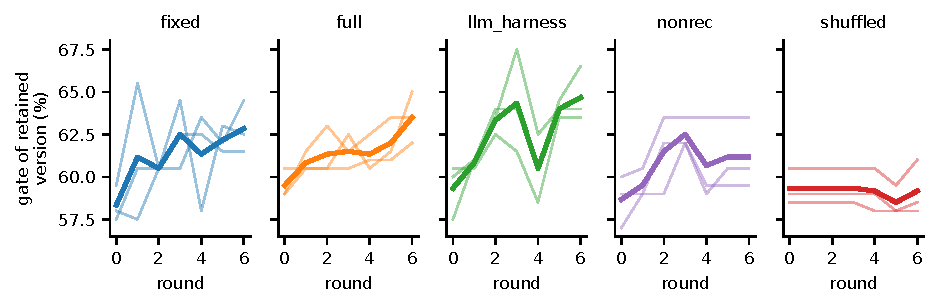
\includegraphics[width=\textwidth]{fig_gates}
  \caption{\textbf{Gate success of the retained policy by round} (cloud platform; thin lines are seeds 1--3, the thick line their mean). A dot marks a round that accepted a new version; every round is scored on 200 newly drawn placements, so a retained version's score can fall from one round to the next. The number in each panel is the change of the mean from round 0 to round 6. With a real verifier and recursive practice the loop climbs 4--5 points at the gate within six rounds; without the verifier (\texttt{shuffled}) it stays flat, and with practice from the frozen initial policy (\texttt{nonrec}) it stops after round 3. Gate gains overstate test gains by the winner's curse (\cref{tab:arms}).}
  \label{fig:gates}
\end{figure*}

\begin{table}[t]
  \centering
  \small
  \caption{\textbf{Per-arm finals} (\%, mean of the 3-evaluation finals over seeds 1--3; seed-0 runs listed separately). Reference 58.9 (Y) / 58.4 (A).}
  \label{tab:arms}
  \resizebox{\linewidth}{!}{%
  \begin{tabular}{@{}lcccccc@{}}
    \toprule
    & \texttt{fixed} & \texttt{full} & \texttt{llm$\ast$} & \texttt{nonrec} & \texttt{shuf.} & \texttt{onebig} \\
    \midrule
    Y, s1--3 & 60.6 & 60.2 & 59.9 & 59.1 & 58.9 & 59.1 \\
    A, s1--3 & 59.1 & -- & 60.1 / 60.2 & -- & -- & -- \\
    A, s0 & 57.2 & -- & -- & 54.8 & 57.5 & 62.7 \\
    \bottomrule
  \end{tabular}}\\[2pt]
  {\footnotesize $\ast$ Y: \texttt{llm\_harness}; A: \texttt{llm} / \texttt{llm\_harness\_cap}.}
\end{table}

\textbf{Finding 2: at six rounds the gains are small, and verified, recursive practice is where they come from.} Every gated run ends within noise of its start or above it (finals 57.1--62.2\% against a reference of 58.4--58.9\%; \cref{tab:arms}); the typical gain is one to two points, the best single seed gains $+3.3$ $[+0.1, +6.6]$, and the registered improvement claim R1 comes to $+1.71$ $[-0.76, +4.23]$ against a $+5$ bar (\cref{tab:goal}). The two largest ingredients are recursion (R3 $+1.72$ $[-0.28, +3.68]$, just under its $+2$ bar) and the verifier (R2 $+1.22$): without a real verifier the loop ends where it started. At the gate (\cref{fig:gates}) the separation is visible within six rounds; at twelve it reaches the sealed tests (Finding 1).

\subsection{Is self-training safe? The gate}
\label{sec:rq2}

\textbf{Finding 3: the gate is what keeps self-training from collapsing.} The behaviour-cloning recipe of \cref{sec:rq3} collapses from 58.5\% to 5.5\% on held-out placements when its versions are accepted unconditionally (\cref{fig:teaser}b); under fresh paired gates the same recipe does not fall below its start beyond noise on the sealed test, and no gated run of the main study does. The gate is cheap (one extra evaluation per candidate) but noisy: a 200-episode paired comparison has a standard deviation of about 3.4 points, so it accepts and rejects many candidates by chance. Its protection relies on recursive practice: over twelve rounds a chain of gate-accepted \texttt{nonrec12} versions drifts below its start (Finding 1).

\subsection{Can the system improve its own training procedure? The meta level}
\label{sec:rq3}

\paragraph{A recipe that fails.} The meta level can be told apart from RL only where RL's recipe fails. One such case was found before any meta-level run: behaviour cloning on the policy's own temperature-1.6 samples with a unit-temperature likelihood collapses when its versions are accepted unconditionally. The repair is a one-knob change (the BC temperature, the sampling temperature or the update operator), and all three knobs are in the harness space, but the meta level is never told which. A registered study starts from this recipe with arms \texttt{fixed} (the gate alone), \texttt{full} (numeric search) and \texttt{llm\_harness} (same compute), four seeds, and the bar S1 $=$ \texttt{llm\_harness} $-$ \texttt{fixed} $\ge +3$, CI above 0.

\begin{figure*}[t]
  \centering
  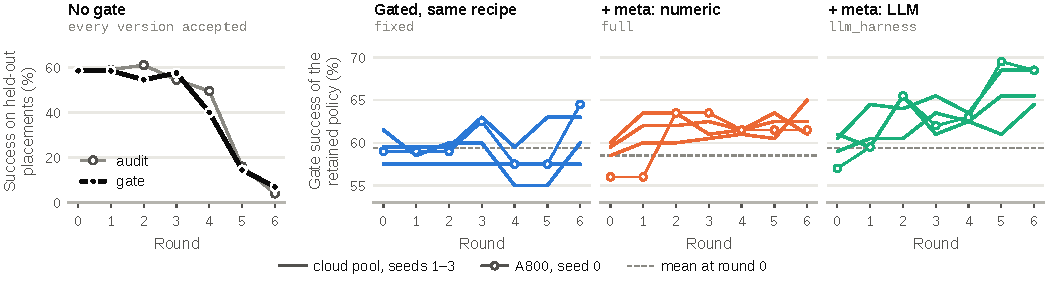
\includegraphics[width=\textwidth]{fig_selfrepair}
  \caption{\textbf{Self-repair study, gate level.} Left: the starting BC recipe collapses when every version is accepted. Right (narrower scale): under the gate the same recipe stays at its starting level (\texttt{fixed}); both proposers find repairs; at the gate the LLM arm looks 4--8 points ahead, on the sealed test it is $+2.65$ (\cref{tab:selfrepair}).}
  \label{fig:selfrepair}
\end{figure*}

\begin{table}[t]
  \centering
  \small
  \caption{\textbf{Self-repair study}: gate / sealed-test final (\%, three evaluations) of each retained version, and what changed. S1 $=$ \texttt{llm\_harness} $-$ \texttt{fixed} $= +2.65$ $[+0.73, +4.58]$ (bar $+3$ missed); S2 $=$ \texttt{llm\_harness} $-$ \texttt{full} $= +1.15$ $[-0.63, +2.92]$; S3 $=$ \texttt{llm\_harness} $-$ hand-tuned GRPO loop $= +0.28$ $[-1.43, +1.97]$.}
  \label{tab:selfrepair}
  \resizebox{\linewidth}{!}{%
  \begin{tabular}{@{}llll@{}}
    \toprule
    seed & \texttt{fixed} (gate only) & \texttt{full} (numeric) & \texttt{llm\_harness} \\
    \midrule
    1 (Y) & 60.0 / 56.1 & 62.5 / 56.7 & 65.5 / 60.1, GRPO in r1 \\
    2 (Y) & start / 58.7, all refused & 65.0 / 59.9, GRPO & 68.5 / 61.3, GRPO in r1 \\
    3 (Y) & 63.0 / 57.5 & 61.0 / 60.2, BC rollout-$T$ & 64.5 / 57.9, BC $T$ 1.6$\to$1.3 \\
    0 (A) & 64.5 / 57.4 & 61.5 / 58.8 & 68.5 / 60.9, GRPO in r2 \\
    \bottomrule
  \end{tabular}}
\end{table}

\textbf{Finding 4: the meta level diagnoses and repairs a failing training procedure on its own.} On all four seeds the language model's first-round diagnosis names the mismatch between the sampling and likelihood temperatures and the missing failure signal (verbatim in the released logs), and its first proposal is the same: switch to GRPO on mixed-outcome scenes at a lower temperature. The gate kept that switch in round 1--2 on three seeds and refused it twice on the fourth, where the model repaired BC instead (\cref{tab:selfrepair}). The repaired loop then gains what the hand-tuned loop gains: S1 $= +2.65$ points $[+0.73, +4.58]$ over the gate alone, positive on three seeds with the interval above zero, and level with the hand-tuned GRPO loop (S3 $= +0.28$ $[-1.43, +1.97]$), while the gate alone holds the policy at its start ($-2.37$ $[-4.12, -0.62]$ against the hand-tuned loop). Two qualifications are registered. S1 is under its $+3$ bar, so the claim is not made in its registered form. And numeric search over the same knobs also finds a repair, on two seeds and only in round 6, ending $1.15$ points behind ($[-0.63, +2.92]$): the model's advantage is speed and reliability of the diagnosis, not a better end point. Six gate-only pilots with extreme GRPO and BC recipes found no second failing scenario.

\textbf{Finding 5: on a recipe that already works, the meta level finds nothing to repair.} All four meta-level arms of the main study land within $\pm 1.2$ points of \texttt{fixed} (R4, \cref{tab:goal}). A second registered study (``v2'') gives the model per-task gate rates with their noise and compares it with a \emph{replica} arm that trains the identical recipe at the same compute: $-0.27$ $[-2.53, +2.00]$ (cloud, seeds 1--3) and $+0.30$ $[-1.60, +2.15]$ (A800, seeds 0--3). The records show why. The model's diagnoses are correct (an unsolved task gives GRPO no signal, another is saturated, the remaining gate changes are noise) and its edits are those a practitioner would try, but its proposals scored $-1.2$ points against the incumbent at the gate ($n{=}30$) where replicas scored $+0.6$ (sd 3.4, $n{=}36$): \emph{every recipe in the space reaches the same plateau}, so there is nothing for a correct diagnosis to fix.

\subsection{Against plain RL at equal compute}
\label{sec:rl}

\textbf{Finding 6: a strictly gated loop does not beat plain RL on a recipe that works.} One round of plain RL with the whole budget (\texttt{onebig}) matches the six-round loop (R5 $-0.58$ $[-2.12, +0.95]$), ties the twelve-round loop on the official test ($-0.38$) and is $2.7$ points ahead of it on the fresh scenes (\cref{tab:long}). The cost is the gate's strictness: the twelve-round runs kept 6, 9 and 9 of their 12 rounds, a refused round's training is discarded, and most refusals in our records are dips within the gate's own noise. Training without a gate loses no rounds, but has no protection either: without it the BC recipe of \cref{fig:teaser}b collapses.

\subsection{How much of a published VLA-RL number is the test set?}
\label{sec:rq4}

\begin{figure}[t]
  \centering
  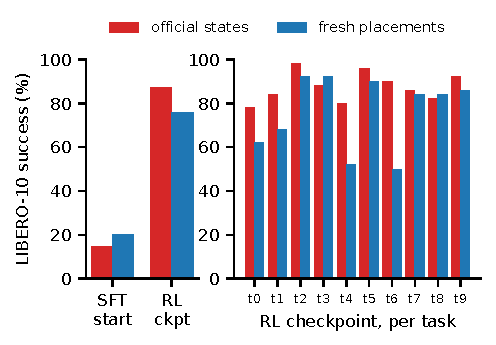
\includegraphics[width=\linewidth]{fig_inflation}
  \caption{\textbf{Train-on-test inflation} (LIBERO-10). Left: official vs.\ fresh placements for the SFT start and the RL checkpoint trained on the official states. Right: the RL checkpoint per task; the loss is concentrated on tasks 4 and 6.}
  \label{fig:inflation}
\end{figure}

\textbf{Finding 7: about a fifth of the headline number.} The released SimpleVLA-RL LIBERO-10 checkpoint was trained by RL on the 50 fixed test states per task. We evaluated it, and its own SFT start, on the 500 official episodes and on 500 placements freshly drawn by LIBERO's own sampler (the same distribution, not a perturbation): SFT 14.6\% official against 20.0\% fresh, RL 87.4\% against 76.0\%. The difference of the two gaps, which cancels any difference in difficulty between the placement sets, is $+16.8$ points $[+9.8, +23.4]$; 500 further never-seen placements give $+16.0$ $[+9.2, +22.4]$ (\cref{fig:inflation}). The method works (the checkpoint gains 56 points on fresh placements), but about a fifth of its headline number is memorisation of the test states.

\section{Discussion}
\label{sec:discussion}
\paragraph{What the evidence does not support.} Two registered bars were missed: the loop's gain over its start ($+3.5$ against $+5$) and the self-repair margin ($+2.7$ against $+3$); at six rounds no ingredient cleared its bar. We do not claim that the loop beats plain RL at equal compute, nor that the language model's diagnosis, rather than the knob space it edits, carries the repair (its margin over blind search is $+1.2$ $[-0.6, +2.9]$).

\paragraph{For practitioners.} A fresh paired gate makes an unsafe recipe safe for one extra evaluation per candidate, but its strictness should match its noise. A single 500-episode evaluation carries about $\pm1.5$ points of noise, so finals should be averaged, and freshly sampled test scenes should complement a fixed list of test states. A language-model meta level pays off only where the recipe can fail.

\paragraph{Limitations.} One simulated benchmark family, one 7B policy and a few-demonstration start; other policies and real robots are untested (real-robot data collection is in progress). Runs interrupted by hardware were continued from a completed round, as the amendments disclose. Preregistration constrains the analysis, not the design: a different recipe space might leave more for a meta level to find.

\section{Conclusion}
\label{sec:conclusion}
Each level of recursive self-improvement does a distinct job for a robot policy: recursion makes it better on unseen scenes, the gate keeps self-training from collapsing, and the meta level repairs a failing training procedure. The effects are modest at this budget, and we report every registered bar we missed; we hope the protocol (sealed tests, fresh scenes, averaged finals, public amendments, one read) outlives the numbers.

{
    \small
    \bibliographystyle{ieeenat_fullname}
    \bibliography{refs}
}
\end{document}
